% !TeX root = tcolorbox.tex
% include file of tcolorbox.tex (manual of the LaTeX package tcolorbox)
\clearpage
\section{初始化选项键}\label{sec:initkeys}%
\tcbset{external/prefix=external/initoptions_}%
\emph{初始化}选项仅适用于基于 |tcolorbox| 及其同类命令生成新环境和新命令的场合。
具体而言，它们可用于
\begin{itemize}
\item\refCom{newtcolorbox}、\refCom{NewTColorBox}、\refCom{NewTotalTColorBox}，
\item\refCom{newtcbox}、\refCom{NewTCBox}、\refCom{NewTotalTCBox}，
\item\refCom{newtcblisting}、\refCom{NewTCBListing}，
\item\refCom{newtcbinputlisting}、\refCom{NewTCBInputListing}，
\item\refCom{newtcbtheorem}、\refCom{NewTcbTheorem}，
\item\refCom{newtcboxfit}、\refCom{NewTCBoxFit}、\refCom{NewTotalTCBoxFit}，
\end{itemize}
以及 \refCom{renewtcolorbox} 等同类命令。

\bigskip
\begin{marker}
通常，这些选项可能会生成计数器等对象。
\textbf{强烈}建议你只在导言区内使用初始化选项。
否则，在使用 \LaTeX 的 |\include| 机制时可能会遇到问题。
此外，建议在加载 \refPkg{hyperref} 之后再用这些选项生成新环境和新命令，
以避免关于\emph{重复标识符}的警告。
\end{marker}


\subsection{带编号的文本框}\label{sec:numberedboxes}
使用初始化选项分配的计数器会被自动管理。特别是，每新建一个文本框，计数器就会递增。


\begin{docCommand}{tcbcounter}{}
  当前带编号文本框的真实计数器名，可在框内使用。
\end{docCommand}

\begin{docCommand}{thetcbcounter}{}
  当前带编号文本框的计数值。可在框内使用，例如在文本框标题中。
  示例参见 \refKey{/tcb/new/auto counter} 及其后续条目。
\end{docCommand}

\begin{docCommand}[doc new=2025-07-21]{tcbcounterof}{\marg{tcolorbox}}
  某个带编号 \meta{tcolorbox} 的真实计数器名。
\end{docCommand}

\begin{docCommand}[doc new=2025-07-21]{thetcbcounterof}{\marg{tcolorbox}}
  由下文所述初始化选项（例如 \refKey{/tcb/new/auto counter}）创建的
  带编号 \meta{tcolorbox} 的计数值。
  \meta{tcolorbox} 可以是已创建的文本框环境名（由 \refCom{newtcolorbox} 等创建），
  也可以是已创建的文本框宏名（由 \refCom{newtcbox} 等创建；此处宏名不带前导反斜杠）。
\end{docCommand}

\begin{docCommand}[doc new=2026-03-05]{renewthetcbcounter}{\marg{tcolorbox}\marg{code}}
  为在某个已存在的 \meta{tcolorbox} 内部使用而重新定义 \refCom{thetcbcounter}。
  多数情况下，这仅用于相当特殊的应用场景。
  \meta{代码}是一段格式化代码，其中应包含 \refCom{tcbcounter} 以引用自动计数器。
  由于该 \meta{代码}会被展开，除 \refCom{tcbcounter} 外，
  每个宏都需用 |\noexpand| 保护。

\begin{dispListing}
\renewthetcbcounter{examplebox}{(Q/\noexpand\thesection/\noexpand\Alph{\tcbcounter})}
\end{dispListing}

另见 \refKey{/tcb/new/number freestyle}。
\end{docCommand}


\clearpage
\begin{newTcbKey}{auto counter}{}{无取值，初始未设置}
  自动创建一个新计数器。
  借助 \refKey{/tcb/new/number format} 与 \refKey{/tcb/new/counter within}，
  可以改变计数器的外观与行为。计数值通过 \refCom{thetcbcounter} 引用。

\inputpreamblelisting{A}

\begin{dispExample}
\begin{pabox}[label={myautocounter}]{Title with number}
This box is automatically numbered with \ref{myautocounter} on page
\pageref{myautocounter}. Inside the box, the \thetcbcounter\ can
also be referenced by |\thetcbcounter|.
The real counter name is \texttt{\tcbcounter}.
\end{pabox}
\end{dispExample}
\end{newTcbKey}


\begin{newTcbKey}{use counter from}{=\meta{tcolorbox}}{无默认值，初始未设置}
  此处复用来自另一个 \meta{tcolorbox} 的计数器。
  注意，\refKey{/tcb/new/number format} 与 \refKey{/tcb/new/counter within}
  的设置会被继承，不能更改。计数值通过 \refCom{thetcbcounter} 引用。

\begin{dispExample}
\newtcolorbox[use counter from=pabox]{mybox}[2][]{%
colback=blue!5!white,colframe=blue!75!black,fonttitle=\bfseries,
title=Some Box \thetcbcounter: #2,#1}

\begin{mybox}[label={myusecounterfrom}]{Title with continued number}
This box is automatically numbered with \ref{myusecounterfrom} on page
\pageref{myusecounterfrom}. Inside the box, the \thetcbcounter\ can
also be referenced by |\thetcbcounter|.
The real counter name is \texttt{\tcbcounter}.
\end{mybox}
\end{dispExample}
\end{newTcbKey}


\clearpage
\begin{newTcbKey}{use counter}{=\meta{counter}}{无默认值，初始未设置}
  此处使用一个普通的已有 \LaTeX\ \meta{计数器}进行编号。
  借助 \refKey{/tcb/new/number format} 与 \refKey{/tcb/new/counter within}，
  可以改变计数器的外观与行为。计数值通过 \refCom{thetcbcounter} 引用。

\begin{dispExample}
% \newcounter{myexample}%  preamble
\newtcolorbox[use counter=myexample,number format=\Alph]{mybox}[2][]{%
colback=green!5!white,colframe=green!55!black,fonttitle=\bfseries,
title=Some Box \thetcbcounter: #2,#1}

\begin{mybox}[label={myusecounter}]{Title with \LaTeX\ number}
This box is automatically numbered with \ref{myusecounter} on page
\pageref{myusecounter}. Inside the box, the \thetcbcounter\ can
also be referenced by |\thetcbcounter|.
The real counter name is \texttt{\tcbcounter}.
\end{mybox}
\end{dispExample}
\end{newTcbKey}


\begin{newTcbKey}[][doc new=2014-09-19]{use counter*}{=\meta{counter}}{无默认值，初始未设置}
  使用一个已存在的 \LaTeX\ \meta{计数器}进行编号。与
  \refKey{/tcb/new/use counter} 不同，\refKey{/tcb/new/number format} 与
  \refKey{/tcb/new/counter within} 这两个选项会被忽略。
  对于已在 |tcolorbox| 宏包之外配置好的计数器（例如标准的
  |figure| 计数器），请使用本选项。
\end{newTcbKey}


\begin{newTcbKey}{no counter}{}{无取值，初始已设置}
  创建的文本框不编号。这是默认值。该选项可用于推翻此前的编号选项。
\end{newTcbKey}


\begin{newTcbKey}[][doc new=2019-10-18]{reset counter on overlays}{\colOpt{=true\textbar false}}{默认 |true|，初始 |false|}
  对于 \refPkg{beamer} 幻灯片，此选项会为文本框计数器调用
  |\resetcounteronoverlays| 命令。在一个帧的后续叠加幻灯片上，
  计数器会自动重置。因此，每个帧的所有幻灯片上计数器取值都相同。
\end{newTcbKey}


\clearpage
\begin{newTcbKeys}[
    doc parameter   = {=\meta{counter}},
    doc description = {无默认值，初始未设置},
  ]{
    {
      doc new         = {2026-03-05},
      doc name        = counter within,
    },
    {
      doc name        = number within,
    },
  }
当 \meta{计数器} 递增时，自动计数器被置零。
此外，在输出时，\meta{计数器} 的值会被加到自动计数器的值之前。\par
若想在自动计数器前加上章号，并在每章新建时重置，可使用：
\begin{dispListing}
counter within=chapter
\end{dispListing}
完整示例参见 \refKey{/tcb/new/Crefname}。
\end{newTcbKeys}


\begin{newTcbKeys}[
    doc parameter   = {=\meta{tcolorbox}},
    doc description = {无默认值，初始未设置},
  ]{
    {
      doc new         = {2026-03-05},
      doc name        = counter within from,
    },
    {
      doc new         = {2025-07-21},
      doc name        = number within from,
    },
  }
这是 \refKey{/tcb/new/counter within}|=|\refCom{tcbcounterof}\meta{tcolorbox} 的快捷写法，
即：当所引用的 \meta{tcolorbox} 的计数器递增时，自动计数器被置零。
\end{newTcbKeys}


\begin{newTcbKey}{number format}{=\meta{format macro}}{无默认值，初始 \texttt{\textbackslash arabic}}
  声明自动计数器的格式。\meta{格式宏}可以是任意有效的 \LaTeX\ 数字格式化宏，
  如 |\arabic|、|\roman| 等。\par
  若想用大写罗马数字显示计数值，可使用：
\begin{dispListing}
number format=\Roman
\end{dispListing}
完整示例参见 \refKey{/tcb/new/auto counter}。
\end{newTcbKey}


\begin{newTcbKey}{number freestyle}{=\meta{code}}{无默认值，初始未设置}
  允许对完整的编号格式进行高级控制。本选项会覆盖由
  \refKey{/tcb/new/counter within} 与 \refKey{/tcb/new/number format} 给出的格式。
  尽管如此，你仍可将它与 \refKey{/tcb/new/counter within} 组合使用，
  以获得所需的重置特性。\par
  \meta{代码}是一段格式化代码，其中应包含 \refCom{tcbcounter} 以引用自动计数器。
  由于该 \meta{代码}会被展开，除 \refCom{tcbcounter} 外，
  每个宏都需用 |\noexpand| 保护。

\inputpreamblelisting{H}

\begin{dispExample}
\begin{phbox}[label={myfreestyle}]{Title with freestyle number}
This box is automatically numbered with \ref{myfreestyle} on page
\pageref{myfreestyle}. Inside the box, the \thetcbcounter\ can
also be referenced by |\thetcbcounter|.
The real counter name is \texttt{\tcbcounter}.
\end{phbox}
\end{dispExample}

若需要在文本框创建\emph{之后}再设置这样的格式，请参见 \refCom{renewthetcbcounter}。
\end{newTcbKey}

\clearpage
\begin{marker}
以下两个选项 \refKey{/tcb/new/crefname} 与 \refKey{/tcb/new/Crefname}
必须在导言区内设置。
注意，\refPkg{cleveref} 的最后一次更新是在 2018 年（截至 2026-03-05），
过去或现在与较新的 \LaTeX\ 内核存在冲突。\refPkg{zref-clever} 是一个可行的替代方案。
\end{marker}

\begin{newTcbKey}[][doc updated=2014-12-01]{crefname}{=\marg{singular}\marg{plural}}{无默认值，初始未设置}
  本选项键只能与需单独加载的 \refPkg{cleveref} 宏包 \cite{cubitt:2018a} 配合使用。
  它为新建的 |tcolorbox| 创建一个交叉引用类型，
  并给出交叉引用的小写 \meta{单数} 与 \meta{复数} 形式。
  该类型即为环境或宏的名称，同时会自动设置 \refKey{/tcb/label type}。
  更多信息参见 \refKey{/tcb/label type} 与 \cite{cubitt:2018a}。
\end{newTcbKey}


\begin{newTcbKey}[][doc updated=2014-12-01]{Crefname}{=\marg{singular}\marg{plural}}{无默认值，初始未设置}
  本选项键只能与需单独加载的 \refPkg{cleveref} 宏包 \cite{cubitt:2018a} 配合使用。
  它为新建的 |tcolorbox| 创建一个交叉引用类型，
  并给出交叉引用的大写 \meta{单数} 与 \meta{复数} 形式。
  该类型即为环境或宏的名称，同时会自动设置 \refKey{/tcb/label type}。
  更多信息参见 \refKey{/tcb/label type} 与 \cite{cubitt:2018a}。
\end{newTcbKey}

\begin{fulldocumentlisting}{
  comment style={raster columns=1,raster left skip=20mm,raster right skip=20mm},
  run pdflatex}
\documentclass[12pt]{article}
\usepackage[papersize={160mm,80mm},noheadfoot,margin=10mm]{geometry}
\usepackage{varioref,cleveref}
\usepackage{tcolorbox}

\newtcolorbox[auto counter,counter within=section,
  crefname={bluebox}{blueboxes}]%
  {mybluebox}[2][]{colback=blue!5!white,colframe=blue!75!black,fonttitle=\bfseries,
     title=Bluebox \thetcbcounter: #2,#1}

\begin{document}
\section{Blue}

\begin{mybluebox}[label={myreference}]{My title}
This is an example.
\end{mybluebox}

\noindent\Cref{myreference}, \cref{myreference}.\\
\Cpageref{myreference}, \cpageref{myreference}.\\
\nameCref{myreference}, \namecref{myreference}.\\
\labelcref{myreference}, \labelcpageref{myreference}.\\
With \texttt{varioref}:\\
\Vref{myreference}, \vref{myreference}.
\end{document}
\end{fulldocumentlisting}



\clearpage

\begin{newTcbKey}[][doc new and updated={2014-09-19}{2023-07-03}]{blend into}{=\meta{name}}{样式，无默认值，初始未设置}
  用于在若干特定情形下，方便地融入已有的命名与编号体系。
  例如，可以用一个 |tcolorbox| 来显示图片并加上标题，
  使其看上去就像标准的 |figure| 环境。
  此处用 \refKey{/tcb/title} 代替标准的 |\caption|，
  用 \refKey{/tcb/list text} 代替标准 |\caption| 的可选参数。
  此外，\refKey{/tcb/new/list type} 会被自动调整（自 6.0.5 版本起更改）。

\meta{name} 的可选值为：
\begin{itemize}
\item\docValue{figures}：融入标准的 |figure| 环境。
\item\docValue{tables}：融入标准的 |table| 环境。
\item\docValue{listings}：融入 \refPkg{listings} 宏包 \cite{hoffmann:listings}
  的标准 |lstlisting| 环境。
  \begin{marker}
  注意，|blend into=listings| 只能在文档正文中使用，
  或更宜放在 |\AtBeginDocument| 子句中！在导言区中不使用
  |\AtBeginDocument| 是不起作用的，因为 |listings| 宏包同样在
  |\AtBeginDocument| 内初始化其计数器。
  \end{marker}
\end{itemize}
\end{newTcbKey}

\enlargethispage*{5cm}
\begin{dispListing}
\begin{figure}[htb]
  \centering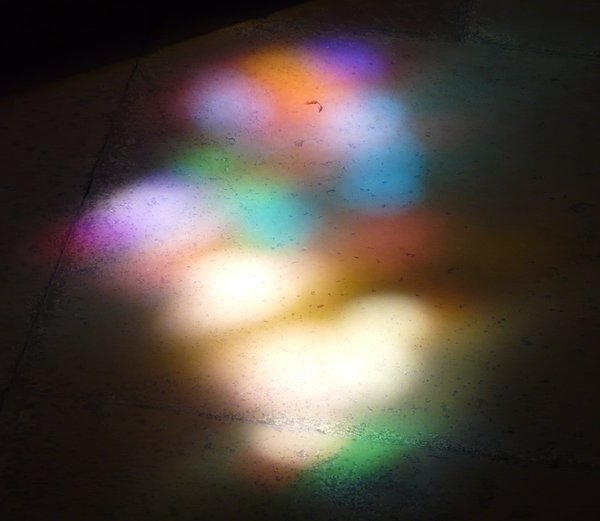
\includegraphics[height=4cm]{lichtspiel.jpg}
  \caption{A standard figure}
\end{figure}

\newtcolorbox[blend into=figures]{myfigure}[2][]{float=htb,capture=hbox,
  title={#2},every float=\centering,#1}

\begin{myfigure}{A tcolorbox figure}
  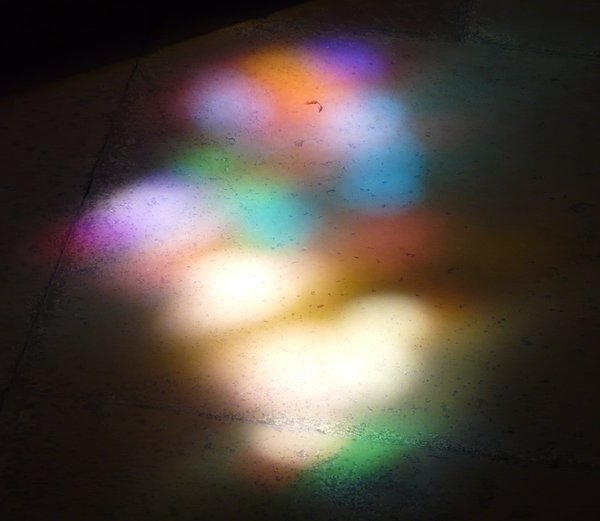
\includegraphics[height=4cm]{lichtspiel.jpg}
\end{myfigure}
\end{dispListing}
{\tcbusetemp}



\clearpage
\begin{docTcbKey}[][doc new=2015-03-13]{blend before title}{=\meta{value}}{无默认值，初始 \docValue{colon}}
  本选项用于设置 \refKey{/tcb/new/blend into} 的标题输出格式。
  注意，这是一个普通的 |tcolorbox| 选项，应当全局设置，
  或放在 \refCom{newtcolorbox} 的常规选项部分中。

\meta{value} 的可选值为：
\begin{itemize}
\item\docValue{colon}：使用 名称/编号 加冒号。
\item\docValue{dash}：使用 名称/编号 加破折号。
\item\docValue{colon hang}：使用 名称/编号 加冒号，并带悬挂缩进。
\item\docValue{dash hang}：使用 名称/编号 加破折号，并带悬挂缩进。
\end{itemize}

\begin{dispListing}
\newtcolorbox[blend into=figures]{myfigure}[2][]{float=htb,capture=hbox,
  blend before title=dash hang,title={#2},every float=\centering,#1}

\begin{myfigure}{A tcolorbox figure with quite a long title}
  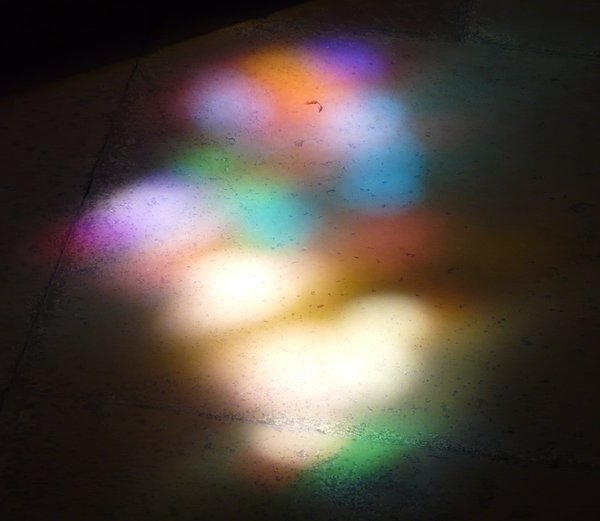
\includegraphics[height=5cm]{lichtspiel.jpg}
\end{myfigure}
\end{dispListing}
{\tcbusetemp}
\end{docTcbKey}

\clearpage
\begin{docTcbKey}[][doc new=2015-03-13]{blend before title code}{=\meta{code}}{无默认值}
  本选项用于设置 \refKey{/tcb/new/blend into} 的标题输出格式。
  \meta{代码}带一个参数，即 名称/编号。
  当 \refKey{/tcb/blend before title} 不够灵活时，可使用本选项。

\begin{dispListing}
\newtcolorbox[blend into=figures]{myfigure}[2][]{float=htb,capture=hbox,
  blend before title code={\fbox{##1}\ },title={#2},every float=\centering,#1}

\begin{myfigure}{A tcolorbox figure}
  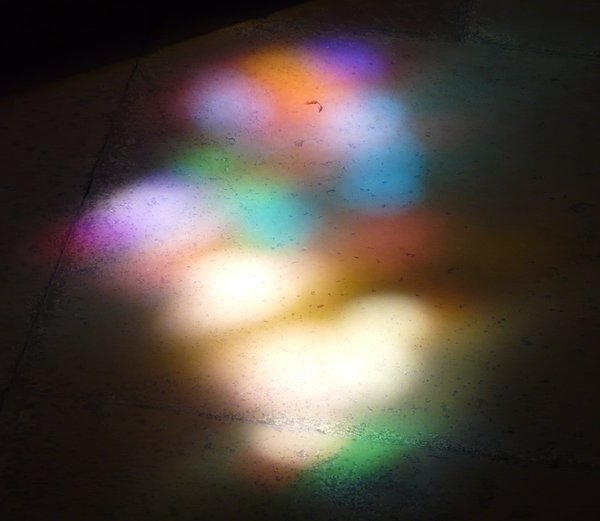
\includegraphics[height=6cm]{lichtspiel.jpg}
\end{myfigure}
\end{dispListing}
{\tcbusetemp}
\end{docTcbKey}



\clearpage
\subsection{\texttt{tcolorbox} 列表}\label{sec:listsof}
对于图和表，\LaTeX\ 提供了 |\listoffigures| 与 |\listoftables| 命令，
用于生成这些编号对象的列表。一个 |tcolorbox| 也可以成为此类列表的一部分。
\begin{enumerate}
\item 通过\emph{初始化}选项 \refKey{/tcb/new/list inside} 指定列表 \meta{名称}。
\item 可选地，通过\emph{初始化}选项 \refKey{/tcb/new/list type}
  为列表条目指定新的 \meta{类型}。
\item 在每个新建的 |tcolorbox| 中，利用上述初始化自动生成列表条目。
  \begin{itemize}
  \item 若设置了 \refKey{/tcb/list entry}，则用它生成条目。
  \item 否则，若设置了 \refKey{/tcb/title}，则用它生成条目。
  \item 再否则，用当前编号与环境名生成条目。
  \end{itemize}
\item 用 \refCom{tcblistof} 显示生成的列表。
\end{enumerate}

\begin{newTcbKey}{list inside}{=\meta{name}}{无默认值，初始未设置}
  为生成的 |tcolorbox| 分配一个列表或目录文件。
  该列表的条目会被保存到一个文件中，文件名扩展名为 \meta{名称}。
  在 \refCom{tcblistof} 中通过该名称引用此列表。
  例如：
\begin{dispListing}
list inside=exam
\end{dispListing}
完整示例参见 \zvref{listing:exercises}。
\end{newTcbKey}


\begin{newTcbKey}{list type}{=\meta{type}}{无默认值，初始 |tcolorbox|}
  可选地，为列表条目指定某个 \meta{类型}。
  对于新的 \meta{类型}，需存在一个宏 |\l@|\meta{类型} 来控制列表条目的格式。
  默认类型由下式定义：
\begin{dispListing}
\newcommand*\l@tcolorbox{\@dottedtocline{1}{1.5em}{2.3em}}
\end{dispListing}
这与 \LaTeX 的 |\l@section| 设置相同。|\l@tcolorbox| 可被重定义，
也可指定新的 \meta{类型}。
\end{newTcbKey}


\clearpage
\begin{docCommand}[doc updated=2021-05-20]{tcblistof}{\oarg{macro}\marg{name}\oarg{short}\marg{title text}}
  显示所给 \meta{名称} 的、由 |tcolorbox| 生成的列表。
  标题由 \meta{宏}\oarg{短标题}\marg{标题文本} 生成，其中 \texttt{\textbackslash section}
  是 \meta{宏} 的默认设置。此处，如通常一样，
  \meta{标题文本}是章节的标题，而 \meta{短标题}是用于页眉和目录的较短标题。
\begin{itemize}
\item 若 \meta{宏} 以 |*| 结尾，\refCom{tcblistof} 会模拟标准 \LaTeX\ 类中
  |\listoffigures| 的行为，并把标题加入左右页眉标记。
\item 若 \meta{宏} 以 |\chapter| 开头，则可能存在的双栏文档设置会被恢复为单栏
  （如同标准 \LaTeX\ 类对 |\listoffigures| 所做的那样）。
\end{itemize}

\medskip
若想在一个小节内部显示列表，可例如：
\begin{dispListing}
\tcblistof[\subsection]{exam}{List of Exercises}
\end{dispListing}
示例结果见 \zvref{listofexercises}。

\medskip
若想像报告或书籍中 |\listoffigures| 那样使用该列表，可例如：
\begin{dispListing}
\tcblistof[\chapter*]{exam}{List of Exercises}
\end{dispListing}

\medskip
若想在默认的 |\section| 设置下为页眉设置短标题，可例如：
\begin{dispListing}
\tcblistof{exam}[List of Exercises]{Elaborate List of Fine Exercises
                                    for all Students of my Course}
\end{dispListing}

\begin{marker}
列表的核心由 |\@starttoc|\marg{名称} 生成，可以把它封装进一个自定义宏。
\end{marker}
\end{docCommand}

\clearpage

\begin{marker}
以下选项并非初始化选项，而是常规选项，
它们通常与 |tcolorbox| 列表配合使用时较为合理。
\end{marker}

\begin{docTcbKey}{list entry}{=\meta{text}}{无默认值，初始未设置}
  若使用本节所述的\flqq tcolorbox 列表\frqq 功能，
  本键用于描述生成列表条目的 \meta{文本}，例如：
\begin{dispListing}
list entry={\protect\numberline{\thetcbcounter}My beautiful Example}
\end{dispListing}
完整示例参见 \zvref{listing:exercises}。\par
若省略 \refCom{thetcbcounter}，\refKey{/tcb/list entry} 也可用于无编号文本框。
\begin{marker}
这是一个定制选项。对于带编号的文本框，通常无需给出
\refKey{/tcb/list entry}，因为该条目会自动生成。
\end{marker}
\end{docTcbKey}

\begin{docTcbKey}[][doc new=2014-09-19]{list text}{=\meta{text}}{样式，无默认值}
  这是把 \refKey{/tcb/list entry} 设为
  |\protect\numberline{\thetcbcounter}|\meta{文本} 的快捷写法。
  因此，以下两种设置等价：
\begin{dispListing}
list text={My beautiful Example},
list entry={\protect\numberline{\thetcbcounter}My beautiful Example}
\end{dispListing}
完整示例参见 \zvref{listing:exercises}。
\end{docTcbKey}

\begin{docTcbKey}{add to list}{=\marg{list}\marg{type}}{无默认值，初始未设置}
  若使用本节所述的\flqq tcolorbox 列表\frqq 功能，列表条目会自动生成。
  借助本键，可以强制向所给 \meta{列表} 添加一个具有所给 \meta{类型} 的条目。
  它会发出：\par
  |\addcontentsline|\marg{列表}\marg{类型}\marg{条目文本}\par
  \meta{条目文本}可由 \refKey{/tcb/list entry} 给出。
\begin{marker}
这是一个定制选项。对于带编号的文本框，本功能会自动配置，
其中 \meta{列表}由 \refKey{/tcb/new/list inside} 设置，
\meta{类型}由 \refKey{/tcb/new/list type} 设置。
\end{marker}
\end{docTcbKey}

